\subsection{Getting on to the System}
\begin{itemize}
	\item{Sign up your account}
	\newline
	You will need to add an account to be able to sign in to the system.
	\begin{figure}[H]
	    	\centering
	    	\fbox{\includegraphics[width=0.5\textwidth]{SignUP}}
	    	\caption{SignUp}
	    	\label{fig:Learning rate 0.1}
   	\end{figure}
	\item{Sign in}
	\newline
	After your account has been created, you will have to sign in.
	\begin{figure}[H]
	    	\centering
	    	\fbox{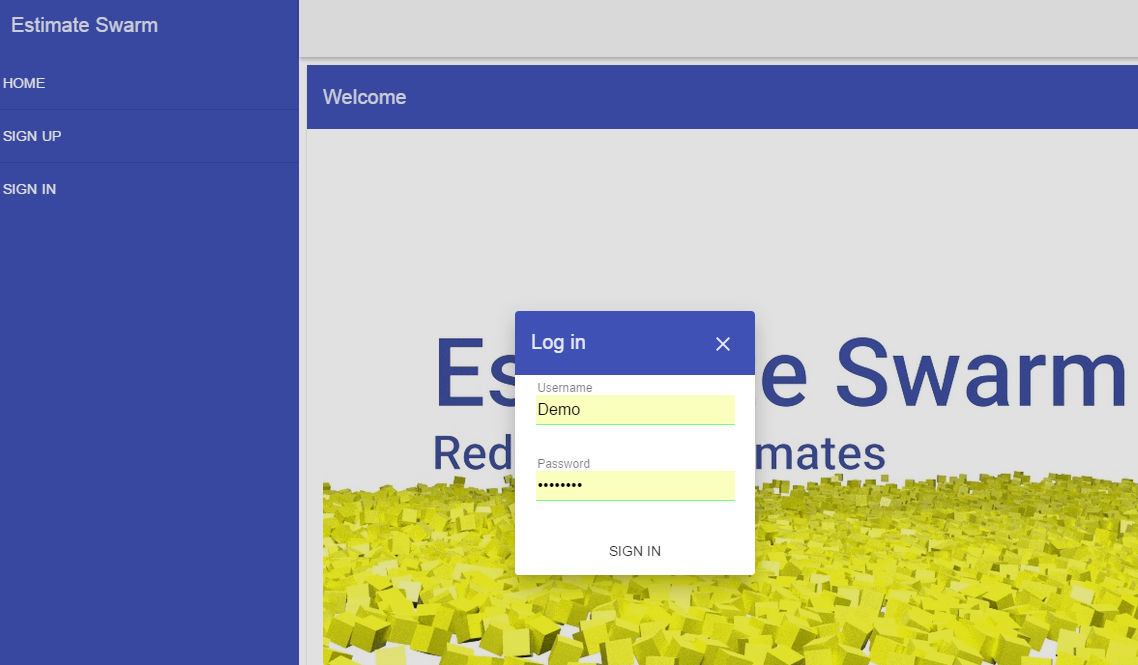
\includegraphics[width=0.5\textwidth]{login}}
	    	\caption{login}
	    	\label{fig:Learning rate 0.1}
   	\end{figure}
\end{itemize}
\subsection{Creating a project}
\begin{itemize}
	\item{Navigate to project list page}
	\newline
	After you have signed in you will be navigated to the projects list page, if you are navigating there from another page, you can simply click on the projects tab on the left side navigation bar.
	\begin{figure}[H]
	    	\centering
	    	\fbox{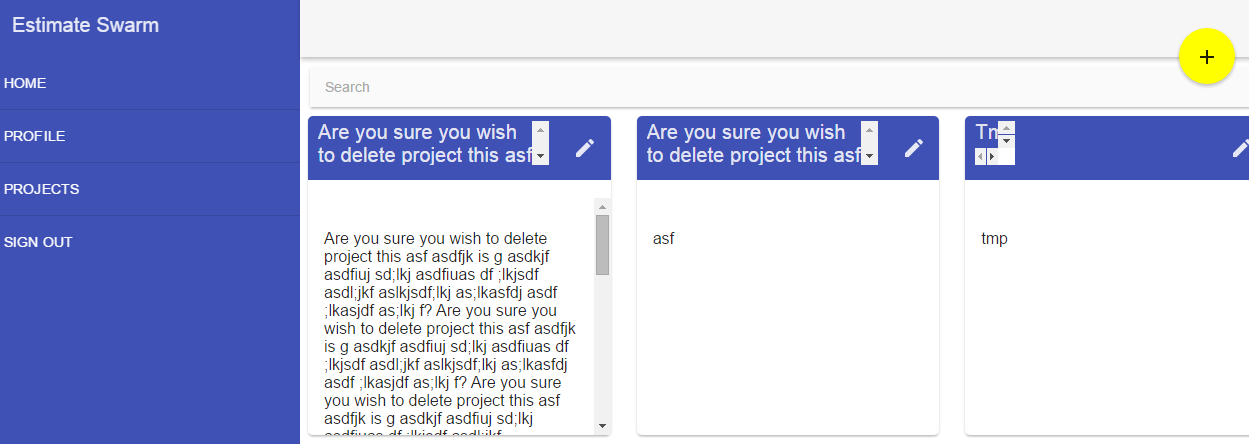
\includegraphics[width=0.5\textwidth]{projectsList}}
	    	\caption{projectsList}
	    	\label{fig:Learning rate 0.1}
   	\end{figure}
	\item{Add a new project}
	\newline
	On the project list page, you can simply click on the "add project" button that is in the top right hand corner of the screen.
	\begin{figure}[H]
	    	\centering
	    	\fbox{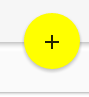
\includegraphics[width=0.5\textwidth]{addButton}}
	    	\caption{addButton}
	    	\label{fig:Learning rate 0.1}
   	\end{figure}
	\item{Add a new project}
	\newline
	On the project list page, you can simply click on the "add project" button that is in the top right hand corner of the screen.
	\begin{figure}[H]
	    	\centering
	    	\fbox{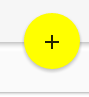
\includegraphics[width=0.5\textwidth]{addButton}}
	    	\caption{addButton}
	    	\label{fig:Learning rate 0.1}
   	\end{figure}
\end{itemize}